% Tea-time talk: Claude-based classification of Socratic math hints
% Build:  tectonic tea_time_talk.tex   (or pdflatex, run twice)
% Figures are read from local copies in outputs_llms/ and outputs/ (Overleaf-ready),
% falling back to ../outputs_llms/ and ../outputs/ -- to regenerate, run the pipeline:
%   uv run socratic-hints all-llm && uv run socratic-hints plot-types-llm
\documentclass[10pt,aspectratio=169,bookmarks=true,bookmarksopen=true,pdfborder={0 0 0},pdfhighlight={/N},linkbordercolor={rgb}{0.5,0.5,0.5},implicit=false,colorlinks=true,urlcolor=blue]{beamer}

\usetheme{Madrid}
\usecolortheme{seahorse}
\usepackage{graphicx}
\usepackage{booktabs}
\usepackage{amsmath}
%\usepackage[colorlinks=true, urlcolor=blue]{hyperref}
\graphicspath{{outputs_llms/}{outputs/}{../outputs_llms/}{../outputs/}}

\setbeamertemplate{navigation symbols}{}
\newcommand{\good}[1]{\textcolor{blue}{#1}}
\newcommand{\bad}[1]{\textcolor{red}{#1}}
\newcommand{\hf}{\textcolor{blue}{[f]}}
\newcommand{\hr}{\textcolor{teal}{[r]}}
\newcommand{\hb}{\textcolor{orange}{[b]}}
\newcommand{\he}{\textcolor{purple}{[e]}}

\title[Claude classifications of Socratic hints]{What Changes When an LLM Classifies Socratic Math Hints?}
\subtitle{Hint transitions across domains, Quarfoot problem types, and a look at my own textbook}
\author{Justin Stevens}
\institute{Tea-time talk}
\date{\today}

\begin{document}

\begin{frame}
  \titlepage
\end{frame}

\begin{frame}{Roadmap}
  \tableofcontents
\end{frame}

% ===========================================================================
\section{The dataset and the two taxonomies}
% ===========================================================================

\begin{frame}{The dataset: SocraticMath}
  \begin{columns}[T]
    \column{0.58\textwidth}
    \textbf{Where it comes from}
    \begin{itemize}
      \item Competition problems from the MATH benchmark, each augmented with a
            \emph{chain of Socratic questions} (Ding et al., CIKM 2024:
            LLM-generated conversational math lessons)
      \item One JSON file per problem:
            \texttt{problem}, \texttt{level} (1--5), \texttt{type},
            \texttt{solution}, \texttt{socratic\_questions}
    \end{itemize}
    \medskip
    \textbf{Scale}
    \begin{itemize}
      \item 7 domains $\times$ 565--590 problems $=$ \textbf{4{,}043 problems}
      \item \textbf{31{,}613 Socratic questions} ($\approx$ 7.8 per problem)
    \end{itemize}
    \column{0.38\textwidth}
    \begin{center}
      \small
      \begin{tabular}{lr}
        \toprule
        domain & problems \\
        \midrule
        algebra & 576 \\
        counting \& probability & 584 \\
        geometry & 575 \\
        intermediate algebra & 565 \\
        number theory & 583 \\
        prealgebra & 590 \\
        precalculus & 570 \\
        \midrule
        total & 4{,}043 \\
        \bottomrule
      \end{tabular}
    \end{center}
  \end{columns}
\end{frame}

\begin{frame}{Taxonomy 1: four hint types}
  Goldin, Koedinger \& Aleven (2013) --- plus one extra type for Socratic chains:
  \medskip
  \begin{description}
    \item[\hf~feature-pointing] draws attention to a specific aspect of \emph{this}
          problem \\ {\small ``Notice that these two angles are vertical angles''}
    \item[\hr~principle-stating] supplies a general rule, definition, or theorem \\
          {\small ``Vertical angles are equal in measure''}
    \item[\hb~bottom-out] directly advances the solution --- set up, substitute, solve \\
          {\small ``Add these two known angles to find the missing one''}
    \item[\he~extension] pushes past the current problem --- applications, generalizations \\
          {\small ``Can you think of other situations where this matters?''}
  \end{description}
  \medskip
  Goal: learn a $4\times4$ \textbf{transition matrix} $M$ per domain, where $p_{ij}$ is
  the probability the next hint is type $j$ given the current one is type $i$.
\end{frame}

\begin{frame}{A worked example (algebra \texttt{hint\_0})}
  \small
  Let
  $f(x)=\begin{cases} ax+3 & x>2\\ x-5 & -2\le x\le 2\\ 2x-b & x<-2 \end{cases}$
  \quad Find $a+b$ if $f$ is continuous.
  \medskip
  \begin{enumerate}\footnotesize
    \item \hf~Can you explain what a piecewise function is and how it is represented algebraically?
    \item \hr~How would you determine if the function is continuous where different pieces meet?
    \item \hf~What conditions need to be satisfied for a piecewise function to be continuous?
    \item \hb~Can you identify the value of $a$ and $b$ that would make the function continuous?
    \item \hb~How would you approach solving for $a$ and $b$?
    \item \hb~Are there any restrictions or constraints on the values of $a$ and $b$?
    \item \he~Can you explain the significance of continuity in real-life applications?
    \item \he~Can you think of other examples where continuity is important?
  \end{enumerate}
  \medskip
  \normalsize
  Labels shown are my hand labels from the report. On this chain
  \good{Claude reproduces all 8/8} (the regex rubric got 7/8, reading \#3 as bottom-out).
\end{frame}

\begin{frame}{Taxonomy 2: Quarfoot's nine problem types}
  A musical metaphor, ordered (roughly) least $\to$ most mathematical substance:
  \medskip
  \begin{center}
    \small
    \begin{tabular}{llp{0.6\textwidth}}
      \toprule
      & type & what it is \\
      \midrule
      FN & First Notes & one-step, single-path, algorithmic; fluency \\
      AC & Accidentals & looks routine, hides a twist; targets a misconception \\
      CH & Chords & one idea, several steps; deepens a single concept \\
      ET & Etudes & drills one technique; word-problem dressing \\
      IM & Improvisations & a playground; first attempts fail, so you experiment \\
      IN & Interpretations & wide-open solution space; compare qualitatively different paths \\
      FP & First Pieces & first problems needing multiple ideas plus a macro-level plan \\
      SP & Showpieces & very hard, hinges on a flash of insight; cognitive \\
      MP & Masterpieces & many skills converging on a generalizable truth; capstones \\
      \bottomrule
    \end{tabular}
  \end{center}
\end{frame}

\begin{frame}{The nine types, illustrated from my number theory textbook}
  Claude's classification of \emph{Olympiad Number Theory} problems (533 total), one example each:
  \begin{center}
    \footnotesize
    \begin{tabular}{lp{0.66\textwidth}l}
      \toprule
      type & problem & source \\
      \midrule
      FN & Find $x$ such that $1+x+x^2+x^3+\cdots=4$. & Mandelbrot \\
      AC & Show there are no integers $x,y$ with $1691x+1349y=1$. & Ch.\ 5 \\
      CH & The sum of 18 consecutive positive integers is a perfect square. Find the smallest possible such sum. & AMC 12 \\
      ET & Compute $\sum_{m=1}^{75}(2+3m)$. & Ch.\ 1 \\
      IM & Pages numbered $1$--$n$; one page number was accidentally added twice, giving $1986$. Which page? & AIME \\
      IN & Prove these Fibonacci identities \emph{in two different ways}. & Ch.\ 2 \\
      FP & Find the 8th term of $1440, 1716, 1848,\ldots$, formed by multiplying corresponding terms of two arithmetic sequences. & AIME \\
      SP & Evaluate $\prod_{n=2}^{\infty}\frac{n^3-1}{n^3+1}$. & Putnam \\
      MP & Prove every positive integer is a sum of non-consecutive Fibonacci numbers. & Zeckendorf \\
      \bottomrule
    \end{tabular}
  \end{center}
\end{frame}

% ===========================================================================
\section{Method and infrastructure}
% ===========================================================================

\begin{frame}{Method: one Claude call per problem, two classifications}
  \begin{itemize}
    \item \texttt{claude-opus-4-8} receives the problem, difficulty level, worked
          solution, and the numbered Socratic chain, and returns strict JSON:
    \begin{enumerate}
      \item one hint label (\texttt{f/r/b/e}) per question, in order
      \item one Quarfoot type for the whole problem
    \end{enumerate}
    \item Prompt contains both taxonomies' definitions + the worked example above as
          the single few-shot anchor
    \item Every response is \textbf{validated} (label count $=$ question count, legal codes
          only) and retried on failure --- batch retry, then per-problem retry
    \item Downstream analysis is \emph{unchanged} from the regex pipeline:
          Dirichlet--multinomial posterior per group, row-averaged KL, similarity $e^{-KL}$
    \item Everything mirrors the old layout:
          \texttt{classifications\_llms/}, \texttt{outputs\_llms/}
  \end{itemize}
\end{frame}

\begin{frame}{Infrastructure: written by Claude, run on Claude}
  \begin{columns}[T]
    \column{0.52\textwidth}
    \textbf{Built with Claude Code}
    \begin{itemize}
      \item Agent wrote the backend, classifier, CLI commands, and plots inside the
            existing \texttt{uv} project
      \item Backend auto-selects: Anthropic SDK if an API key is set, else headless
            \texttt{claude -p} calls on my Claude subscription
      \item Batched 10 problems/call ($\approx$ 410 calls), 12 parallel workers
    \end{itemize}
    \column{0.44\textwidth}
    \textbf{Robustness (needed it!)}
    \begin{itemize}
      \item Resumable: each problem's JSON written on arrival; re-runs skip finished work
      \item Circuit breaker: 3 consecutive all-fail batches $\Rightarrow$ stop
            (usage limit), auto-resume later
    \end{itemize}
  \end{columns}
  \bigskip
  \textbf{Compute \& cost}
  \begin{itemize}
    \item Throughput $\approx$ 53 problems/min $\Rightarrow$ $\approx$ \textbf{80 min of active compute}
          for all 4{,}043 problems ($\approx$ 3 h wall clock: hit the subscription usage limit twice, auto-resumed)
    \item Marginal cost: \textbf{\$0} on the subscription
          ($\approx$ \$60 API-equivalent at Opus list prices)
  \end{itemize}
\end{frame}

\begin{frame}{Claude and the regex rubric disagree --- a lot}
  \begin{itemize}
    \item Hint labels (MATH): agreement on only \textbf{65.0\%} of 31{,}613 questions
    \item Quarfoot types (MATH): \textbf{30.9\%} of 4{,}043 problems
    \item Quarfoot types (my book): \textbf{25.3\%} of 533 problems --- consistent story
  \end{itemize}
  \smallskip
  \begin{center}
    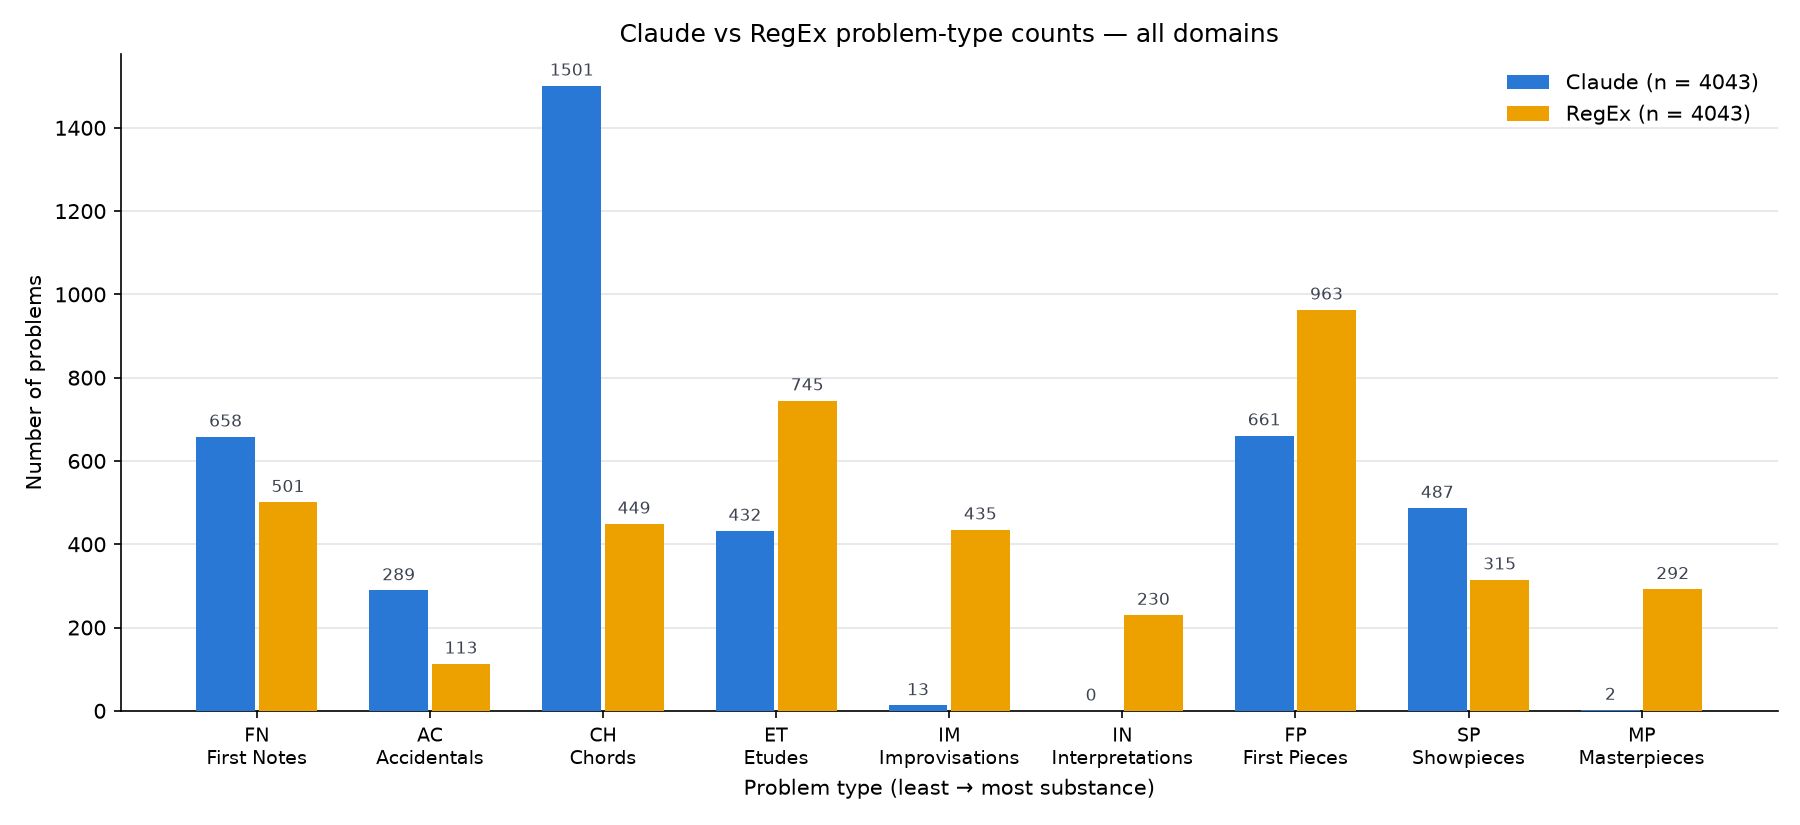
\includegraphics[height=0.52\textheight]{problem_type_hist_llm_vs_regex.png}
  \end{center}
  \smallskip
  Claude concentrates problems in \textbf{Chords} (1{,}501 vs.\ 449) and nearly abandons the
  open-solution-space types: IM 13, IN 0, MP 2 (regex: 435 / 230 / 292).
\end{frame}

% ===========================================================================
\section{Results: which domains differ, and why}
% ===========================================================================

\begin{frame}{How one similarity entry is computed (Claude labels)}
  \footnotesize
  Count transitions, add the all-ones Dirichlet prior, normalize rows --- e.g.\ the
  counting \& probability $f$-row has counts $(491,147,495,40)$, so
  $p_{ff}=\frac{491+1}{1173+4}\approx 0.418$. Doing this for both domains:
  \begin{align*}
    M_{\text{algebra}}=\begin{pmatrix}
      0.227 & 0.224 & 0.498 & 0.051\\
      0.160 & 0.272 & 0.502 & 0.067\\
      0.089 & 0.158 & 0.600 & 0.153\\
      0.030 & 0.073 & 0.193 & 0.704
    \end{pmatrix}
    \quad
    M_{\text{count.\ \& prob.}}=\begin{pmatrix}
      \mathbf{0.418} & 0.126 & 0.421 & 0.035\\
      0.184 & 0.242 & 0.441 & 0.133\\
      0.070 & 0.104 & 0.715 & 0.111\\
      0.030 & 0.060 & 0.079 & \mathbf{0.831}
    \end{pmatrix}
  \end{align*}
  Row-by-row symmetrized KL, then average over the four rows:
  \begin{center}
    \begin{tabular}{lcccc|c}
      \toprule
      row & $f$ & $r$ & $b$ & $e$ & mean \\
      \midrule
      $\tfrac12\!\left[KL(A\|C)+KL(C\|A)\right]$ & \textbf{0.096} & 0.030 & 0.030 & 0.063 & \textbf{0.0549} \\
      \bottomrule
    \end{tabular}
  \end{center}
  \smallskip
  Similarity $=e^{-0.0549}\approx 0.947$ --- the \emph{lowest} of any pair under Claude labels.
  The $f$-row does the most work: c\&p chains feature-pointing $\to$ feature-pointing
  at almost \textbf{2$\times$} algebra's rate (0.418 vs.\ 0.227).
\end{frame}

\begin{frame}{The outlier domain flips: geometry $\to$ counting \& probability}
  \begin{columns}[T]
    \column{0.5\textwidth}
    \centering RegEx labels \\
    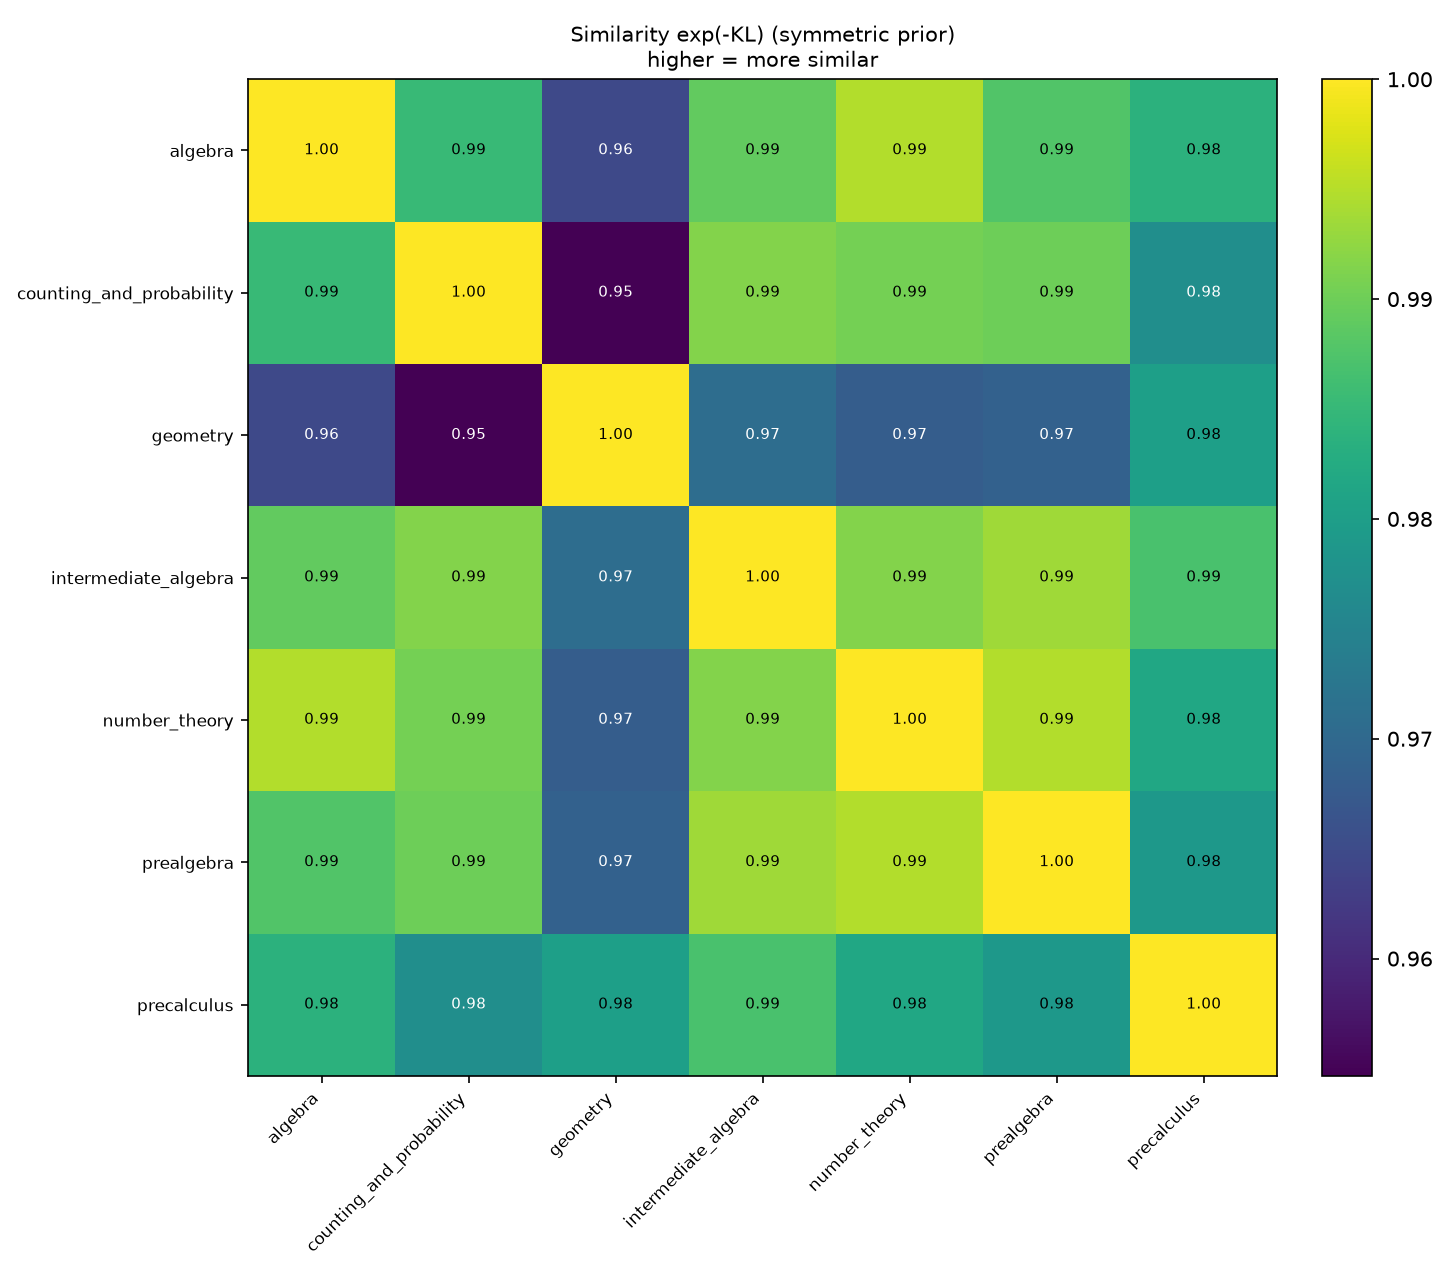
\includegraphics[height=0.58\textheight]{outputs/similarity_symmetric.png}
    \column{0.5\textwidth}
    \centering \textbf{Claude labels} \\
    
\includegraphics[height=0.58\textheight]{similarity_symmetric.png}
  \end{columns}
  \smallskip
  \begin{itemize}
    \item RegEx: geometry most dissimilar from everything (the report's conclusion)
    \item Claude: geometry is among the \emph{most central} domains (mean sim.\ 0.981);
          \textbf{counting \& probability} is the outlier (mean sim.\ 0.958)
  \end{itemize}
\end{frame}

\begin{frame}{Why counting \& probability reads differently}
  \begin{itemize}
    \item Its hint \emph{marginals} already stand out --- most feature-pointing, least
          principle-stating of any domain:
      \begin{center}
        \small
        \begin{tabular}{lcccc}
          \toprule
          & f & r & b & e \\
          \midrule
          counting \& probability & \textbf{23.9\%} & \textbf{13.9\%} & 50.0\% & 12.1\% \\
          all domains (mean)      & 18.9\% & 18.6\% & 51.5\% & 10.9\% \\
          \bottomrule
        \end{tabular}
      \end{center}
    \item And its \emph{dynamics}: hints stack observations
          ($f\to f$ at $0.418$) before computing, and once a chain reaches extensions
          it stays there ($e \to e$ at $0.831$ vs.\ $0.704$ for algebra)
    \item Intuition: ``notice how many ways\ldots'' beats ``recall the theorem\ldots'' ---
          combinatorics hints scaffold by \emph{observation}, not by \emph{principle}
  \end{itemize}
  \medskip
  \textbf{Takeaway:} with better labels, the geometry-outlier result looks like an artifact
  of the keyword rubric.
\end{frame}

% ===========================================================================
\section{Results: my textbook vs.\ MATH number theory}
% ===========================================================================

\begin{frame}{Same classifier, two corpora: MATH number theory vs.\ book ch.\ 1--10}
  \begin{center}
    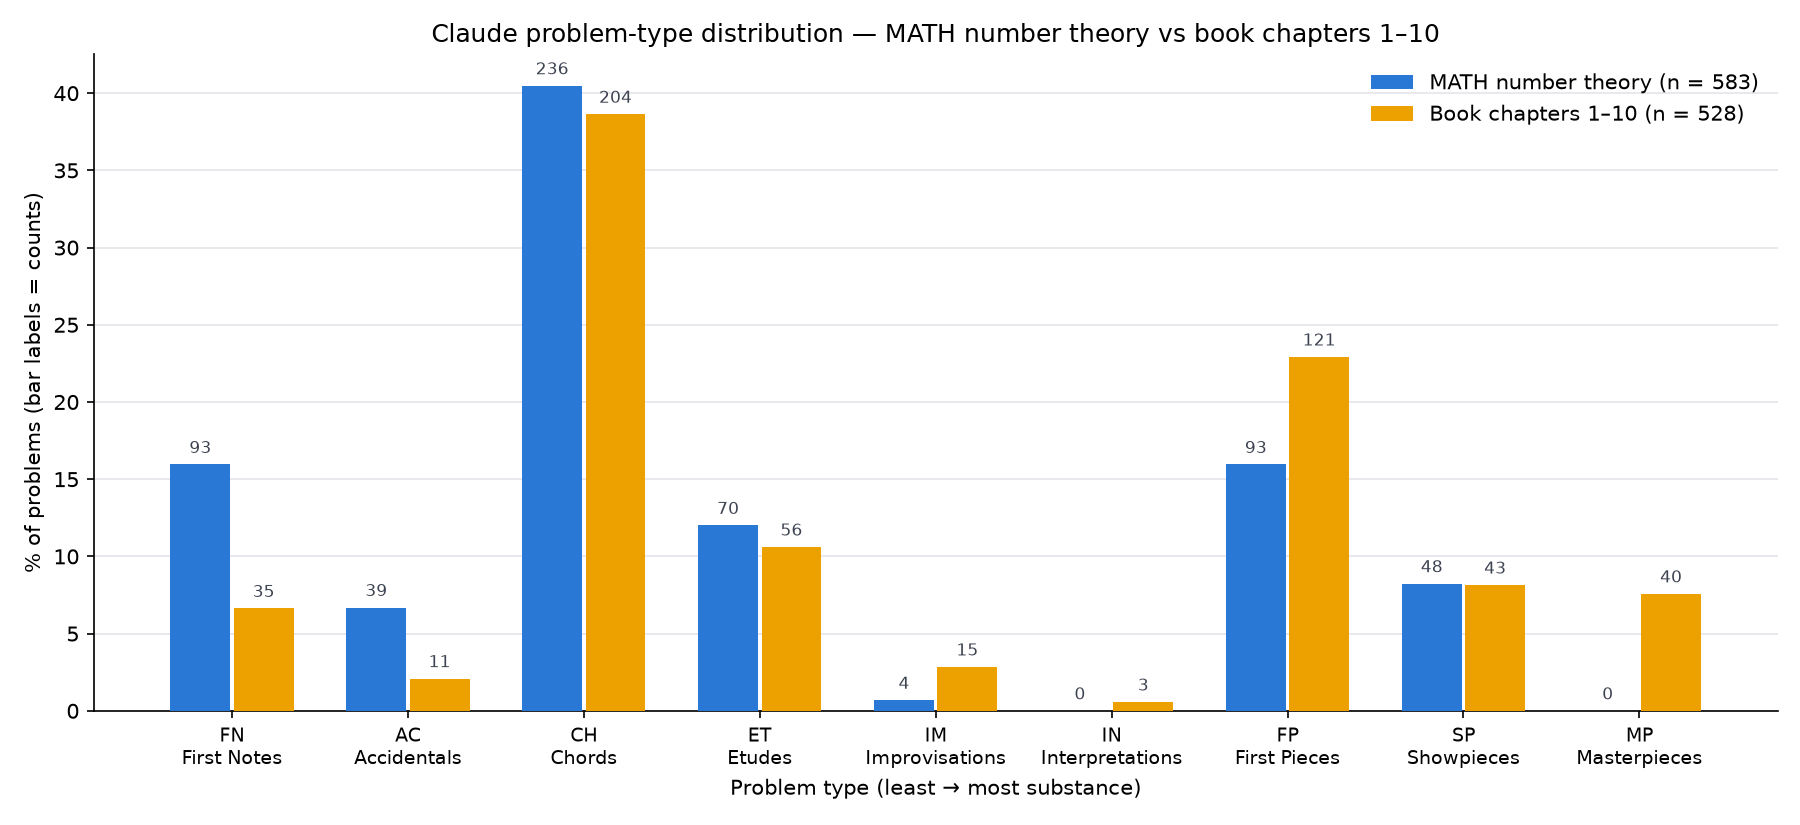
\includegraphics[height=0.6\textheight]{problem_type_hist_number_theory_vs_book.png}
  \end{center}
  \begin{itemize}
    \item The \emph{middles} match: Chords 40.5\% vs.\ 38.6\%; Etudes and Showpieces within
          $\sim$1.5 points
    \item The \emph{tails} diverge in opposite directions
  \end{itemize}
\end{frame}

\begin{frame}{Reading the tails as pedagogy}
  \begin{columns}[T]
    \column{0.5\textwidth}
    \textbf{MATH number theory} (n = 583)
    \begin{itemize}
      \item Thick floor of fluency checks: FN + AC = \textbf{22.6\%}
            (``what is the units digit of\ldots'')
      \item \bad{Zero Masterpieces} (2 in all 4{,}043 MATH problems)
      \item A competition \emph{item bank}
    \end{itemize}
    \column{0.5\textwidth}
    \textbf{Book chapters 1--10} (n = 528)
    \begin{itemize}
      \item Light on drills: FN + AC = 8.7\%
      \item More multi-idea planning: FP 22.9\% vs.\ 16.0\%
      \item \good{7.6\% Masterpieces} --- culminating capstones (Zeckendorf, USAMO, Putnam)
      \item A curated \emph{learning arc}
    \end{itemize}
  \end{columns}
  \bigskip
  The arc is visible \emph{within} the book too: the share of high-substance problems
  (FP/SP/MP) climbs from \textbf{24\%} in Ch.\ 1 to $\approx$ \textbf{50\%} by Ch.\ 9--10.
  \smallskip

  \textbf{Why this is credible:} identical classifier, prompt, and rubric on both corpora ---
  near-identical middles, sharply different tails $\Rightarrow$ properties of the corpora,
  not classifier noise.
\end{frame}

% ===========================================================================
\section{Pedagogy and takeaways}
% ===========================================================================

\begin{frame}{What this offers people who write textbooks}
  \begin{itemize}
    \item \textbf{An audit tool for your problem mix.} Type profiles make the shape of a
          book quantitative: drills vs.\ concept-deepeners vs.\ capstones, per chapter and
          overall --- and comparable against item banks or other texts.
    \item \textbf{A check on the arc.} You can verify the substance axis actually climbs
          the way you intended (mine does: 24\% $\to$ 50\% high-substance).
    \item \textbf{Gap-finding.} What I learned about my own book:
      \begin{itemize}
        \item essentially no \emph{Interpretations} (3 of 533) --- almost nowhere do I ask
              students to solve one problem \emph{two different ways} and compare
        \item Improvisations are rare too (15) --- few low-stakes ``playground'' problems
        \item the capstones I hoped were there really do register (40 Masterpieces)
      \end{itemize}
    \item \textbf{For tutoring systems:} hint scaffolding should adapt per domain ---
          combinatorics wants observation-chaining, algebra wants principle-then-compute.
  \end{itemize}
\end{frame}

\begin{frame}{Takeaways, caveats, next steps}
  \textbf{Takeaways}
  \begin{enumerate}
    \item LLM labels change the science: the domain outlier flips from geometry to
          counting \& probability, with an interpretable mechanism
    \item Problem-type profiles act as corpus fingerprints: item bank vs.\ curated arc
    \item The whole pipeline is cheap enough to be a routine tool ($\approx$ 80 min, \$0 marginal)
  \end{enumerate}
  \medskip
  \textbf{Caveats}
  \begin{itemize}
    \item No human-labeled evaluation set yet --- the earlier ``gold set'' was itself
          LLM-authored, so I dropped it; a real one is the top priority
    \item Claude saw the worked solution: single-solution write-ups may bias it against
          open-ended types (IM/IN) and Masterpieces
    \item One model, one prompt --- no inter-rater $\kappa$ yet
  \end{itemize}
  \medskip
  \textbf{Next steps:} human gold set + Cohen's $\kappa$ with a second annotator;
  hint transitions vs.\ difficulty level; HMM over noisy labels; blind the classifier
  to the solution text as a robustness check.
\end{frame}

\begin{frame}
  \centering
  {\Large Thanks! Questions?}

  \bigskip
  \small
  Code available \href{https://github.com/justinstevens42/SocraticMath}{here}.
\end{frame}

\end{document}
